\documentclass{beamer}
%\usetheme{Ilmenau}
%\usecolortheme{beaver}

\usepackage[slovak,american]{babel}
\usepackage[utf8]{inputenc}
\usepackage{graphicx}
\usepackage{adjustbox}
 \usepackage{xcolor}
 
 \newsavebox\MBox
\newcommand\Cline[2][red]{{\sbox\MBox{$#2$}%
  \rlap{\usebox\MBox}\color{#1}\rule[-2.2\dp\MBox]{\wd\MBox}{1pt}}}

%\usefonttheme{serif}

%\definecolor{UKOrange}{HTML}{ef9424} %
\definecolor{UKOrange}{HTML}{7a2c18} %
\definecolor{UKBrown}{HTML}{a96d5e} %
\definecolor{UKLight}{HTML}{d8b6ab} %
\definecolor{UKDark}{HTML}{7a4f44}
\definecolor{UKDarker}{HTML}{4d312b} 
\definecolor{UKDarkest}{HTML}{2e1e1a}
\definecolor{UKRed}{HTML}{bf1f1c}

\setbeamertemplate{footline}[frame number]{}
\setbeamertemplate{navigation symbols}{}

%\usecolortheme{beaver}
\setbeamertemplate{itemize item}[square]
\setbeamercolor{itemize item}{fg = UKBrown}
\setbeamercolor{itemize subitem}{fg = UKLight}
\setbeamercolor{enumerate item}{fg = UKDark}

\setbeamercolor{footnote}{fg=UKLight}
\setbeamercolor{footnote mark}{fg=UKLight}
\setbeamerfont{footnote}{size=\tiny}
\renewcommand\footnoterule{}

\usetheme{default}
\beamertemplatenavigationsymbolsempty
\setbeamercolor{title}{fg=white, bg=UKBrown}
\setbeamercolor{frametitle}{fg=white, bg=UKBrown}
\setbeamercolor{block title}{bg=UKBrown, fg= white}
\setbeamercolor{block body}{bg =UKLight, fg = UKDarkest}

\setbeamercolor{block title alerted}{bg=UKOrange, fg= white}
\setbeamercolor{block body alerted}{bg =UKLight, fg = UKDarkest}


%\setbeamercolor{section in toc}{fg = UKBrown}
%\setbeamercolor{section in toc}{fg = UKDarkest}

% odstrani gulicky
\renewcommand*{\slideentry}[6]{}

\useoutertheme[subsection=false]{miniframes}
\AtBeginSection[]{\subsection{}}

\setbeamercolor{below lower separation line head}{bg=UKDark}
\addtobeamertemplate{headline}{}{%
  \begin{beamercolorbox}[colsep=0.5pt]{below lower separation line head}
  \end{beamercolorbox}
}
%\setbeamercolor*{mini frame}{fg=white,bg=UKRosy}
\setbeamercolor{section in head/foot}{fg=UKLight, bg=UKDark}

\usepackage{etoolbox}
\makeatletter
\preto{\@verbatim}{\topsep=0pt \partopsep=0pt }
\makeatother

%\setbeamertemplate{itemize/enumerate body begin}{\normalsize}
%\setbeamertemplate{itemize/enumerate subbody begin}{\normalsize}




%\newcommand{\codeblock}[2]{ \begin{block}{#1} \begin{verbatim}#2\end{verbatim}\end{block}}

%\defbeamertemplate*{title page}{customized}[1][]
%{
%  \begin{centering}
%    \begin{beamercolorbox}[sep=8pt,center]{title}
%      \usebeamerfont{title}\inserttitle
%    \end{beamercolorbox}
%  \end{centering}
%  \bigskip
%
%\begin{columns}[onlytextwidth,T]
%
%
%  \column{27mm}
%  \includegraphics[width=27mm]{images/logoFMFI.png}
%  
%  \column{\dimexpr\linewidth-54mm-6mm}
%  \centering
%  \vspace{5mm}  
%  \usebeamerfont{author}\insertauthor\par
%  \vspace{5mm}
%  \usebeamerfont{institute}\insertinstitute\par
%
%  \column{27mm}
%  \includegraphics[width=27mm]{images/logoUK.png}  
%\end{columns}
%\centering
%\vspace{7mm}
%  \usebeamerfont{date}\insertdate\par
%}

\DeclareMathOperator*{\argmin}{arg\,min}
\newcommand{\e}[1]{$\cdot 10^{#1}$}

%\newcommand{\codeblock}[2]{ \begin{block}{#1} \begin{verbatim}#2\end{verbatim}\end{block}}

\title[5. cvičenie]{Pokročilé spracovanie obrazu - Histogramy, šum, vyhladzovanie a zostrovanie}
\author[Kocur]{Ing. Viktor Kocur \\{\small viktor.kocur@fmph.uniba.sk}}
\institute{DAI FMFI UK}
\date{29.10.2020}

\begin{document}
\selectlanguage{slovak}

\begin{frame}
  \titlepage
\end{frame}

\section{Jas}
\subsection{Histogram}
\begin{frame}
\frametitle{Histogram}
\begin{block}{imhist}
imhist(I) - zobrazí histogram, v prípade že výstup zapíšeme do premennej, tak nič nevykreslí ale vráti nam vektor s histogramom.
\end{block}

\begin{block}{Úloha}
Preveďte zatisie.jpg na šedotónový obrázok. Na jeho histograme sú tri peaky. Upravte obrázok, tak aby pixely približne patriace len jednému z peakov boli úplne biele, ostatné nechajte tak.
\end{block}
\end{frame}

\subsection{Úpravy jasu}
\begin{frame}
\frametitle{Úprava jasu}
\begin{block}{Gamma korekcia}
Kontrast v obraze môžeme meniť pomocou gamma korekcie: $i_{out} = A \cdot i^{\gamma}$, kde $i$ predstavuje jas jednotlivých pixelov obrázka. Pozor jas musí byť medzi 0 a 1!
\end{block}

\begin{block}{Lineárne roztiahnutie}
Pre linárne roztiahnutie môžeme použiť nasledujúcu úpravu:
\begin{equation*}
i_{out} = \frac{i - min (I)}{max(I) - min(I)},\end{equation*}
kde i sú hodnoty jasu pre jednotlivé pixely a I predstavuje množinu jasov všetkých pixelov. Tiež chceme hodnoty jasu medzi 0 a 1.
\end{block}
\end{frame}

\begin{frame}
\frametitle{Ekvalizácia histogramu}
\begin{block}{Ekvalizácia}
Ekvalizácia histogramu je metóda, ktorá mení jas v obraze tak, aby výsledný histogram vyzeral čo najrovnomernejšie.
\end{block}

\begin{block}{histeq}
histeq(I) - vráti obrázok po ekvalizácii histogramu.
\end{block}

\begin{block}{Úloha}
Pre obrázok krajinka.png vyskúšajte rôzne metódy úpravy kontrastu. Po úpravách si zobrazte obrázky aj histogramy.
\end{block}
\end{frame}

\subsection{Prahovanie}
\begin{frame}
\frametitle{Prahovanie}
\begin{block}{imbinarize}
imbinarize(I) - vráti binarizovaný obraz s prahom určeným Otsuho metódou.
\end{block}

\begin{block}{imbinarize}
imbinarize(I, t) - vráti binarizovaný obraz s prahom t.
\end{block}

\begin{block}{Úloha}
Vyskúšajte prahovanie na obrázkoch coins.png, qr.jpg a zatisie.jpg.
\end{block}
\end{frame}

\begin{frame}
\frametitle{Adaptívne prahovanie}
\begin{block}{imbinarize}
imbinarize(I, 'adaptive') - vráti binarizovaný obraz s použitím adaptívneho prahovania.
\end{block}

\begin{block}{Úloha}
Vyskúšajte adaptívne prahovanie na obrázku coins.png a qr.jpg.
\end{block}
\end{frame}

\section{Šum}
\subsection{Gaussovský aditívny šum}
\begin{frame}
\frametitle{Šum}
\begin{block}{Ako vzniká šum?}
Šum môže vzniknúť vo viacerých fázach získania obrazu. Napríklad už pri reakcii sezoru na svetlo, alebo pri prenose informácie. 
\end{block}

\begin{block}{Prečo je nutné modelovať šum?}
V reálnych situáciách sa šumu nevyhneme, preto je vhodné mať k dispozícii model šumu, aby sme ho vedeli potlačiť.
\end{block}
\end{frame}

\begin{frame}
\frametitle{Gaussovský aditívny šum}
\begin{block}{Aditivita}
Šum je aditívny ak pláti $I = I_{orig} + S$.
\end{block}

\begin{block}{Gaussovovský charakter šumu}
\begin{equation}
P(S_{i,j} = x) = \frac{1}{\sigma \sqrt{2\pi}} e^{-\frac{(x-\mu)^2}{2\sigma^2}}
\end{equation}
\end{block}

\noindent\makebox[\textwidth]{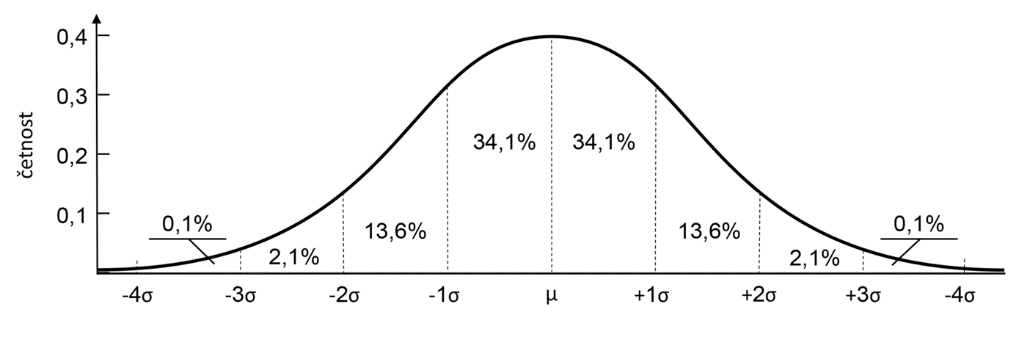
\includegraphics[width=0.9\linewidth]{gauss.png}}
\end{frame}

\begin{frame}
\frametitle{Gaussovský aditívny šum - matlab}
\begin{block}{randn}
randn(sz) - vráti maticu veľkosti sz (napr. sz = size(I)) s náhodnými prvkami z gaussovskej distribúcie s $\sigma = 1$ a $\mu = 0$.
\end{block}

\begin{block}{Úloha}
Vytvorte funkciu zasum(I,sigma), ktorá obraz I (predpokladajte, že je šedotónový a v double) zašumí šumom s $\mu = 0$ a $\sigma = \sigma$. Ošetrite výstup tak, aby bol obraz v rozmedzí medzi 0 a 1. Otestujte funkciu na obrázku. Použite rôzne sigma.
\end{block}
\end{frame}

\subsection{Salt and Pepper}
\begin{frame}
\frametitle{Salt and Pepper}
\begin{block}{Salt and Pepper}
Salt and pepper (sol a korenie) šum nastáva vtedy ak sa jeden pixel zmení buď na úplne tmavý, alebo úplne svetlý.
\end{block}

\begin{block}{rand}
rand(sz) - vráti maticu veľkosti sz, jej prvky majú náhodné hodnoty z rovnomernej distribúcie medzi 0 a 1.
\end{block}


\begin{block}{Úloha}
Vytvorte funkciu okoren(I,p1,p2), ktorá šedotónový obraz I (predpokladajte, že je v double) zašúmí, tak že s pravdepodobnosťou p1 dostaneme úplne biely pixel a s pravdepodobnosťou p2 dostaneme úplne tmavý pixel. Funkciu otestujte pre rôzne parametre.
\end{block}
\end{frame}


\section{Vyhladzovanie}
\subsection{Priemerovanie}
\begin{frame}
\frametitle{Vyhladzovanie}
\begin{block}{Prečo vyhladzujeme}
Pri pozorovaní jemne zašumeného obrazu okom je stále jednoduché pozorovat' ho a porozmiet' jeho obsahu. V spracovaní obrazu a počítačovom videní však niektoré algoritmy môžu jednoducho zlyhať. Preto je nutné potlačiť šum. To dosiahneme vyhladzovaním.
\end{block}
\end{frame}

\begin{frame}
\frametitle{Konvoúcia}
\begin{block}{Konvolúcia - integrálna verzia - reálne čísla}
\begin{equation*}
J= I \ast M \iff J (\chi, \psi) = \int_{-\infty}^{\infty}\int_{\infty}^{\infty} I(x,y)M(\chi - x,\psi - y) dx dy
\end{equation*}
\end{block}

\begin{block}{Konvolúcia - diskrétna verzia - reálne čísla}
\begin{equation*}
J = I \ast M \iff J(r,c) = \sum_{u=-\infty}^{\infty}\sum_{v=-\infty}^{\infty} I(u,v)M(r-u,c-v)
\end{equation*}
\end{block}

  \begin{alertblock}{Pozor}
  Pre príklad obrazov predpokladáme, že $I$ a $M$ majú nulové hodnoty všade kde je index mimo rozmerov obrazu.
  \end{alertblock} 

\end{frame}

\begin{frame}
\frametitle{Konvolúcia}
\noindent\makebox[\textwidth]{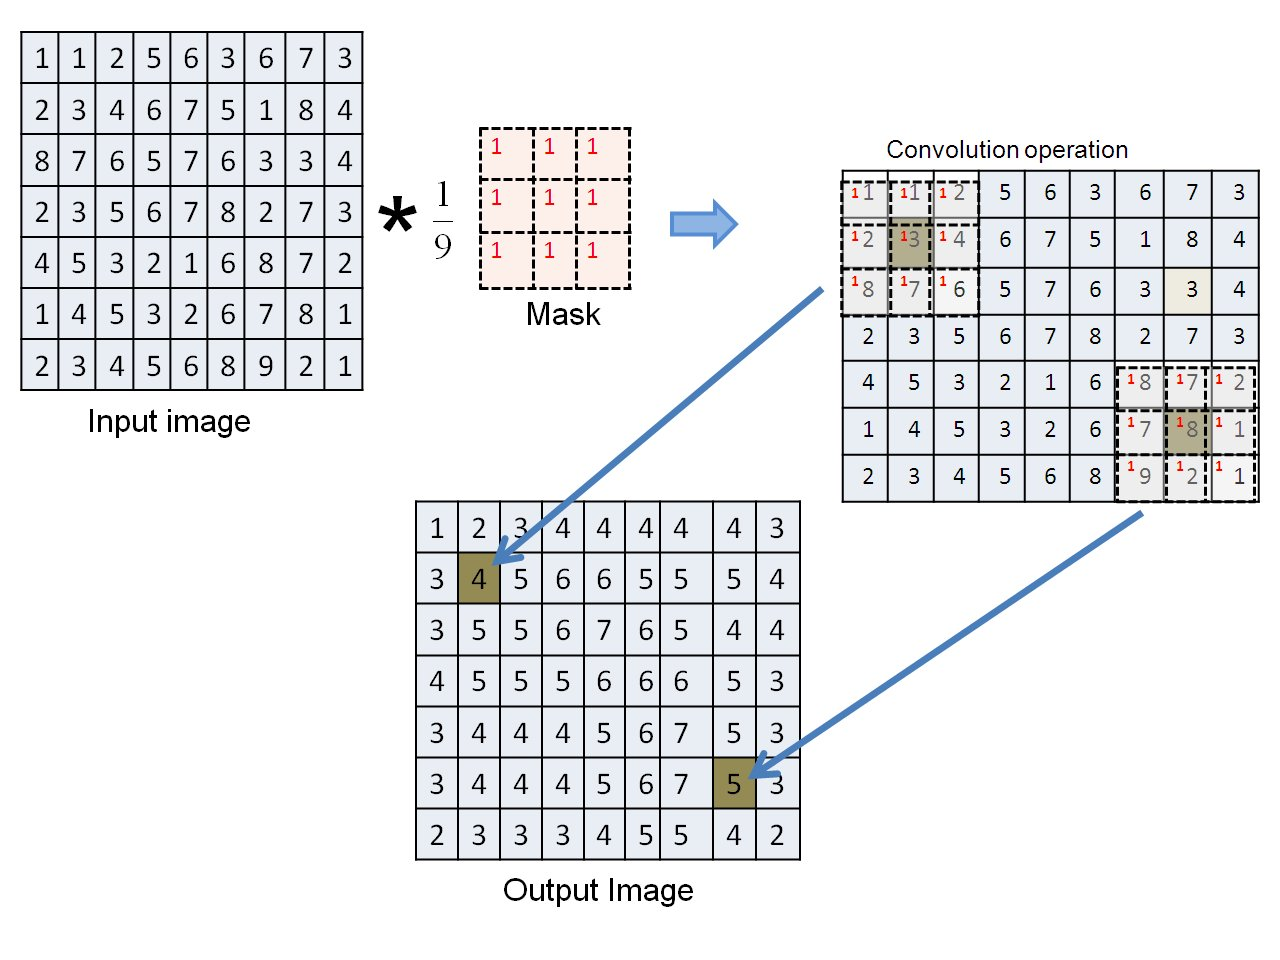
\includegraphics[width=0.9\linewidth]{convolution.jpg}}
\end{frame}

\begin{frame}
\frametitle{Konvolúcia - matlab}
\begin{block}{conv2}
conv2(A,B) - realizuje kovnolúciu matice A s maticou B
\end{block}

\begin{block}{imfilter}
imfilter(I,f) - konvolučne prefiltruje obraz I filtrom (maticou) f.
\end{block}

\begin{block}{imfilter}
imfilter(I,f, 'option') - option upravuje veľkosť výsledného obrzu (napr. 'same'), alebo to čo sa bude brať za hodnoty ak filter 'siahne' mimo (napr. 'replicate', 'symmetric'). Môžete použiť aj viac options naraz.
\end{block}
\end{frame}

\begin{frame}
\frametitle{Konvolúcia - filtre}
\begin{block}{Ručne}
Filtre môžeme vyrobiť aj ručne napr. priemerovací filter je ones(3)/9.
\end{block}

\begin{block}{fspecial}
fspecial('name', params) - vráti filter podľa mena 'name' a parametrov.
\end{block}

\begin{block}{fspecial}
fspecial('average',hsize) - vráti priemerovací filter veľkosti hsize \\
fspecial('gaussian',hsize,sigma) - vráti gaussovský filter veľkosti hsize a strednou hodnotou sigma
\end{block}
\end{frame}

\begin{frame}
\frametitle{Konvolúcia - filtre}
\begin{block}{Úloha}
Zobrazte si gaussovský filter pre rôzne sigma a veľkosti.
\end{block}

\begin{block}{imgaussfilt}
imgaussfilt(I, sigma) - prefiltruje obraz I gaussovským filtrom, je to obdobné ako kombinácia fspecial a imfilter, ale je efektívnejšia.
\end{block}

\begin{block}{Úloha}
Zašumte si obrázok aditívnym šumom a skúste ho vyhladiť rôznymi gaussovým a priemerovacím filtrom. To isté spravte pre salt and pepper. Otestujte aj rôzne parametre šumu.
\end{block}
\end{frame}

\begin{frame}
\frametitle{Konvolúcia - filtre}
\begin{block}{Úloha}
Zobrazte si gaussovský filter pre rôzne sigma a veľkosti.
\end{block}

\begin{block}{imgaussfilt}
imgaussfilt(I, sigma) - prefiltruje obraz I gaussovským filtrom, je to obdobné ako kombinácia fspecial a imfilter, ale je efektívnejšia.
\end{block}

\begin{block}{Úloha}
Zašumte si obrázok aditívnym šumom a skúste ho vyhladiť rôznymi gaussovým a priemerovacím filtrom. To isté spravte pre salt and pepper. Otestujte aj rôzne parametre šumu.
\end{block}
\end{frame}

\subsection{Mediánová filtrácia}
\begin{frame}
\frametitle{Mediánová filtrácia}
\begin{block}{Mediánová filtrácia}
Na šum typu salt and pepper nefunguje priemerovanie. Preto je vhodnejšie využiť iný postup. Namiesto priemerovania budeme pre každé okno používať medián.
\end{block}

\begin{block}{medfilt2}
medfilt2(I, [m n]) - vráti obraz po mediánovej filtrácii oknom veľkosti m $\times$ n.
\end{block}

\begin{block}{Úloha}
Zašumte si obrázok aditívnym šumom a skúste ho vyhladiť mediánovým filtrom. To isté spravte pre salt and pepper.
\end{block}
\end{frame}

\section{Ostrenie obrazu}
\subsection{Unsharp Masking}

\begin{frame}
\frametitle{Unsharp masking - Princíp} 
\noindent\makebox[\textwidth]{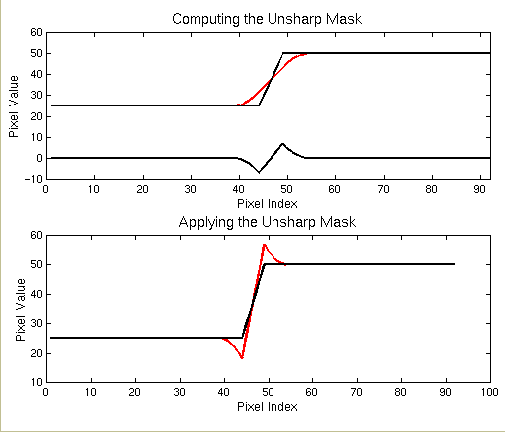
\includegraphics[width=0.9\linewidth]{unsharp.png}}
\end{frame}

\begin{frame}
\frametitle{Unsharp masking} 
  \begin{block}{Ostrenie}
    Máme obrázok, ktorý je rozostrený. Chceme ho vyostriť. Táto úloha sa dá pochopiť aj ako zvýrazňovanie hrán.
  \end{block} 
 
  \begin{block}{Unsharp masking - princíp}
    $I_{ostr\acute{y}} = I_{origin\acute{a}l} + p \cdot \left( I_{origin\acute{a}l} - I_{vyhladen\acute{y}} \right)$
  \end{block}
  
  \begin{block}{Úloha}
  Vytvorte funkciu unsharp\_mask(I,p,sigma), ktorý aplikuje unsharp masking s parametrom p na obrázok I pomocou gaussovho vyhladenia s hodnotou sigma. Aplikujte na blurred.pgm.
  \end{block}
\end{frame}
\end{document}